\subsection{Trigger}
\label{sec:enujjTrigger}

Events in the \enujj~channel are selected online using unprescaled single electron or electron-\MET-jet-jet triggers  
triggers.  Each component of these triggers (e.g. electrons, jets, and PFMHT) is referred to as a ``leg''.
The exact trigger used depends on the run period.  
The full list of triggers for the \enujj~channel and their 
associated run periods are listed in Table~\ref{tab:enujjSingleEleElectronHadHLT}. 

\begin{table}
  \begin{center}
    \scriptsize
    \begin{tabular}{l|c} 
      HLT path & Run number range \\
      \hline\hline
      \multicolumn{2}{c}{Run2011A} \\
      \hline
      \verb HLT_Ele27_CaloIdVT_CaloIsoT_TrkIdT_TrkIsoT_v1  & 160404--161176  \\%& 5.281 \\
      \verb HLT_Ele27_CaloIdVT_CaloIsoT_TrkIdT_TrkIsoT_v2  & 161216--163261  \\%& 28.321 \\
      \verb HLT_Ele27_CaloIdVT_CaloIsoT_TrkIdT_TrkIsoT_v3  & 163269--163869  \\%& 168.613 \\ 
      \verb HLT_Ele17_CaloIdVT_CaloIsoT_TrkIdT_TrkIsoT_CentralJet30_CentralJet25_PFMHT15_v2  & 165088--165633 \\%& 139.027 \\
      \verb HLT_Ele25_CaloIdVT_CaloIsoT_TrkIdT_TrkIsoT_CentralJet30_CentralJet25_PFMHT20_v4  & 165970--166967 \\%& 524.904 \\
      \verb HLT_Ele22_CaloIdVT_CaloIsoT_TrkIdT_TrkIsoT_CentralJet30_CentralJet25_PFMHT20_v2  & 167039--167913 \\%& 265.747 \\
      \verb HLT_Ele22_CaloIdVT_CaloIsoT_TrkIdT_TrkIsoT_CentralJet30_CentralJet25_PFMHT20_v4  & 170249--173198 \\%& 741.938 \\
      \verb HLT_Ele27_CaloIdVT_CaloIsoT_TrkIdT_TrkIsoT_CentralJet30_CentralJet25_PFMHT20_v2  & 173236--173692 \\%& 246.527 \\
      \hline
      \multicolumn{2}{c}{Run2011B} \\
      \hline
      \verb HLT_Ele30_CaloIdVT_CaloIsoT_TrkIdT_TrkIsoT_DiCentralJet30_PFMHT25_v1    &     175832--178380  \\%& 1698 \\
      \verb HLT_Ele27_WP80_DiCentralPFJet25_PFMHT15_v4 &     178420--179889  \\
      \verb HLT_Ele27_WP80_DiCentralPFJet25_PFMHT15_v5 &     179959--180252  \\
    \end{tabular}
    \caption{HLT paths for \enujj~channel}
    \label{tab:enujjSingleEleElectronHadHLT}    
  \end{center}
\end{table}
    
The names of the triggers listed in Table
\ref{tab:enujjSingleEleElectronHadHLT} correspond to the algorithms
used to reconstruct and identify the objects making up each leg.
For the first period of data taking, up to run 178380, electrons with the identification selection
\texttt{CaloIdVT\_CaloIsoT\_TrkIdT\_TrkIsoT} are used in the trigger with varying \pt~requirements
(the number after the word {\tt Ele} refers to the electron \pt~threshold in GeV).
For the following period, from run 178420 until the end of the data taking, electrons with the identification selection
\texttt {WP80} are used instead.  The explicit cuts used in these electron identification selections are listed in 
Table \ref{tab:electron-trigger-cuts}.

During the period of running between run 165088 and run 178380, jets of type
\texttt{CentralJet} are used in the trigger with varying \pt~requirements
(the number after the words {\tt CentralJet}, {\tt DiCentralJet}, or {\tt DiCentralPFJet} refers to the 
jet \pt~threshold in GeV).
For the following period, from run 178420 until the end of the data taking, jets of type
\texttt{CentralPFJet} are used in the trigger.  
Both types of jets are reconstructed using the \akt~algorithm, and both types of jets
require $|\eta| < 2.6$.
The name \texttt{CentralJet} refers to jets reconstructed from calorimeter
input only.  The name \texttt{CentralPFJet} refers to jets reconstructed with a PF algorithm
that has been simplified from the full offline PF algorithm according to the computing restrictions in the HLT.

\begin{table}
  \centering
  \small
  \begin{tabular}{c|c|c|c|c}
    \multirow{3}{*}{ID name} & Calorimeter & Calorimeter & Track & Track \\
    & isolation & identification & isolation & identification \\
    & requirements & requirements & requirements & requirements  \\
    \hline\hline
    \multirow{2}{*}{{\tt CaloIdVT}} & \HoE$ < 0.05$ (0.05)             & & & \\
                                    & \SigmaiEtaiEta$ <0.011$ (0.031) & & & \\
    \multirow{2}{*}{{\tt CaloIsoT}} & & \EMIso$ < 0.125$  (0.075) & & \\
                                    & & \HADIso$ < 0.125$ (0.075) & & \\
    \multirow{2}{*}{{\tt TrkIdT}}   & & & \dEtaIn$ <0.008$ (0.008) & \\
                                    & & & \dPhiIn$ <0.07$  (0.05)  & \\
    \multirow{2}{*}{{\tt TrkIsoT}}  & & & & \multirow{2}{*}{\TRKIso$ < 0.125$ (0.075)} \\
                                    & & & & \\
    \hline
    \multirow{2}{*}{{\tt WP80}}     & \HoE$<0.04$ (0.025)          & \EMIso$<0.07$ (0.05)   & \dEtaIn$<0.004$ (0.007) & \multirow{2}{*}{\TRKIso$<0.09$ (0.04)} \\ 
                                    & \SigmaiEtaiEta$<0.01$ (0.03) & \HADIso$<0.10$ (0.025) & \dPhiIn$<0.06$ (0.03)   &  \\
  \end{tabular}
  \caption{Electron identification selections applied in the HLT for electrons in the EB (and EE).  
    The values in the ``Electron ID name'' column correspond to parts of the HLT trigger names 
    listed in Table \ref{tab:enujjSingleEleElectronHadHLT}.
    The variables listed here are defined in Section \ref{sec:id-electron}.
  }
  \label{tab:electron-trigger-cuts}
\end{table}

The efficiencies for different objects defining the trigger paths are discussed below.
\begin{itemize}
\item{{\bf Electrons:} } 
  For all of the triggers listed in Table \ref{tab:enujjSingleEleElectronHadHLT}, 
  the electron \pt~requirements are significantly lower than the electron \pt~requirements 
  in the \enujj~preselection, and threshold effects related to electron \pt~are avoided.
  However, the ID and isolation requirements are different between online and offline selection and therefore the 
  trigger efficiency should be checked. 
  The efficiency with which 
  the \texttt{CaloIdVT\_CaloIsoT\_TrkIdT\_TrkIsoT}
  and \texttt {WP80} electron legs select electrons that are identified offline as HEEP electrons 
  was measured by using $\mbox{\PZz} \rightarrow \mbox{ee}$ events. 
  This efficiency averaged over the whole 2011 data taking period is found to be 95.5$^{+1.0\%}_{-3.5\%}$.
  The quoted systematic uncertainties are due to variations observed in the efficiency of the HLT {\tt WP80} identification
  as a function of electron $\eta$ which are not taken into account 
  in this analysis; the statistical uncertainties are negligible.
  The efficiency of the electron leg of the \texttt{HLT\_Ele27\_WP80\_DiCentralPFJet25\_PFMHT15} 
  trigger as a function of electron pseudorapidity is shown in Figure \ref{fig:wp80}.
  Overall, the efficiency was found to be stable as a function of number of pile-up interactions: 
  the small variations observed are well within the systematic uncertainties already quoted above.
  This 4.5\% overall inefficiency is only included in the signal predictions 
  (to correct for the fact that these trigger requirements are not explicitly applied in the MC).
  This inefficiency is not propagated to the major backgrounds, since their 
  normalization is already derived from comparison with data in control regions.
\item{{\bf Jets:} } The \pt~cut on the jets at \enujj~preselection is 40~\GeV, 
  tight enough to avoid trigger threshold bias produced by 
  the jet \pt~requirements online. 
  The jet legs of the triggers in Table \ref{tab:enujjSingleEleElectronHadHLT} are found to be fully efficient.
\item{{\bf PFMHT}: } The \MET~cut at \enujj~preselection is 55~\GeV: tight enough 
  to avoid trigger threshold bias produced by the {\verb PFMHT } requirements online.
  The PFMHT legs of the triggers in Table \ref{tab:enujjSingleEleElectronHadHLT} are found to be fully efficient.
\end{itemize}

\begin{figure}
  \centering
  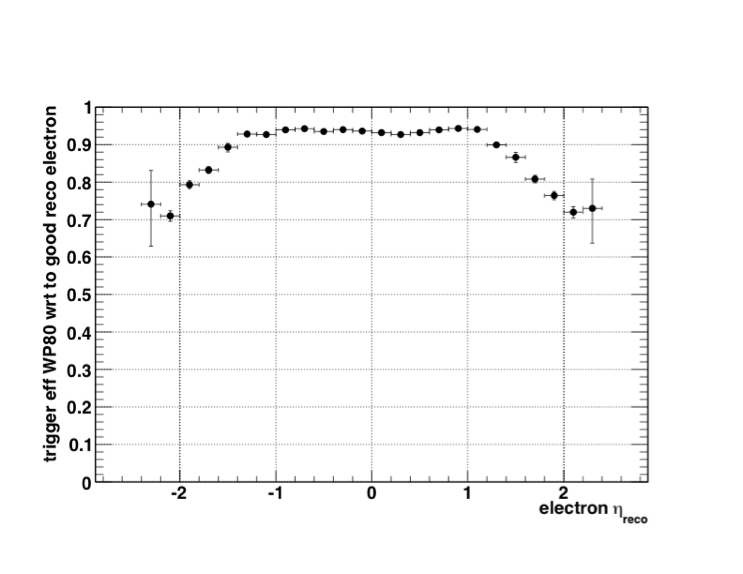
\includegraphics[width=0.60\textwidth]{tex/analysis/event_selection/fig/trigger/wp80_eta.png}
  \caption{
    Efficiency with which the \texttt{Ele27\_WP80} leg of the \texttt{HLT\_Ele27\_WP80\_DiCentralPFJet25\_PFMHT15}
    trigger identifies an electron with $\pt > 40$, if that same electron is identified offline as a HEEP electron.
    The efficiency is shown as a function of electron pseudorapidity.
  }
  \label{fig:wp80}
\end{figure}

